\documentclass[tikz,border=10pt]{standalone}
\usepackage{pgfplots}
\usepackage{pgfplotstable}
\pgfplotsset{compat=1.18}
\begin{document}
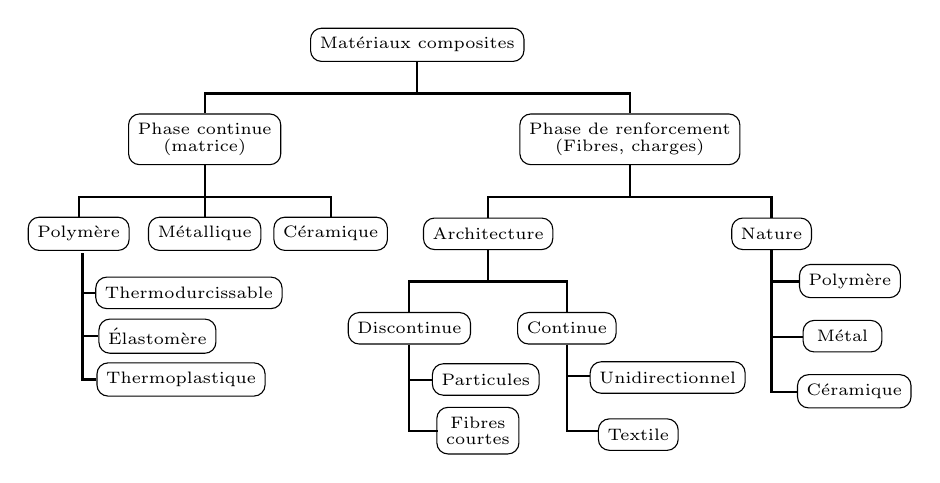
\begin{tikzpicture}[
    every node/.style = {draw, rectangle, rounded corners, align=center,
    minimum width = 1cm, minimum height = 0.4cm,
    font = \fontsize{6}{6}\selectfont, draw = black, fill = white}
  ]    
  % Racine
  \node (root)  {Matériaux composites};
  % Niveau 1
  \node (phaseContinue) at ([yshift = -1.2cm, xshift = -2.7cm] root)
    {Phase continue \\ (matrice)};
  \node (phaseRenforcement) at ([yshift = -1.2cm, xshift = 2.7cm] root)
    {Phase de renforcement \\ (Fibres, charges)};
  % Lignes horizontales et verticales
  \draw[thick] (root.south) -- ++(0,-0.4cm) -| (phaseContinue.north);
  \draw[thick] (root.south) -- ++(0,-0.4cm) -| (phaseRenforcement.north);
  % Niveau 2 - Phase continue
  \node (polymere)   at ([yshift=-1.2cm, xshift=-1.6cm] phaseContinue) {Polymère};
  \node (metallique) at ([yshift=-1.2cm] phaseContinue) {Métallique};
  \node (ceramique)  at ([yshift=-1.2cm, xshift=1.6cm] phaseContinue) {Céramique};
  % Lignes horizontales et verticales
  \draw[thick] (phaseContinue.south) -- ++(0,-0.4cm) -| (polymere.north);
  \draw[thick] (phaseContinue.south) -- ++(0,-0.4cm) -| (metallique.north);
  \draw[thick] (phaseContinue.south) -- ++(0,-0.4cm) -| (ceramique.north);    
  \node (td) at ([yshift=-0.75cm, xshift=1.4cm] polymere) {Thermodurcissable}; % Décalé à droite
  \node (el) at ([yshift=-1.3cm,  xshift=1cm]   polymere) {Élastomère};       % Même xshift
  \node (tp) at ([yshift=-1.85cm, xshift=1.3cm] polymere) {Thermoplastique}; % Même xshift
  % Connexions avec traits diagonaux propres
  \draw[thick] (polymere.east)  ++(-0.6cm,-0.25cm) |- (td.west);  % Ligne en ┐
  \draw[thick] (polymere.east)  ++(-0.6cm,-0.25cm) |- (el.west);   % Même connexion
  \draw[thick] (polymere.east)  ++(-0.6cm,-0.25cm) |- (tp.west);   % Même connexion   
  % Niveau 2 - Phase de renforcement
  \node (architecture) at ([yshift=-1.2cm, xshift=-1.8cm] phaseRenforcement) {Architecture};
  \node (nature)       at ([yshift=-1.2cm, xshift=1.8cm] phaseRenforcement) {Nature};
  % Lignes horizontales et verticales
  \draw[thick] (phaseRenforcement.south) -- ++(0,-0.4cm) -| (architecture.north);
  \draw[thick] (phaseRenforcement.south) -- ++(0,-0.4cm) -| (nature.north);
  % Niveau 3 - Architecture
  \node (discontinue) at ([yshift=-1.2cm, xshift=-1cm] architecture) {Discontinue};
  \node (continue)    at ([yshift=-1.2cm, xshift=1cm]  architecture) {Continue};
  % Lignes horizontales et verticales
  \draw[thick] (architecture.south) -- ++(0,-0.4cm) -| (discontinue.north);
  \draw[thick] (architecture.south) -- ++(0,-0.4cm) -| (continue.north);
  % Niveau 4 - Discontinue
  \node (particules)  at ([yshift=-0.65cm, xshift=0.97cm] discontinue) {Particules};
  \node (fibresCours) at ([yshift=-1.3cm, xshift=0.87cm]  discontinue) {Fibres \\courtes};
  % Lignes horizontales et verticales
  \draw[thick] (discontinue.south) |- ++(0.3cm,-0.45cm) (particules.north);
  \draw[thick] (discontinue.south) |- ++(0.36cm,-1.1cm) (fibresCours.north);
  % Niveau 4 - Continue
  \node (unidirectionnel) at ([yshift=-0.625cm, xshift=1.28cm] continue) {Unidirectionnel};
  \node (textile)         at ([yshift=-1.35cm, xshift=0.907cm] continue) {Textile};
  % Lignes horizontales et verticales
  \draw[thick] (continue.south) |- ++(0.3cm,-0.4cm) (unidirectionnel.north);
  \draw[thick] (continue.south) |- ++(0.4cm,-1.1cm) (textile.north);
  % Niveau 3 - Nature
  \node (metalliqueNature) at ([yshift=-0.6cm, xshift=0.995cm] nature)  {Polymère};
  \node (ceramiqueNature)  at ([yshift=-1.3cm, xshift=0.9cm]   nature)     {Métal};
  \node (polymereNature)   at ([yshift=-2cm,   xshift=1.05cm]  nature) {Céramique};
  % Lignes horizontales et verticales
  \draw[thick] (nature.south) |- ++(0.35cm,-0.4cm)  (metalliqueNature.north);
  \draw[thick] (nature.south) |- ++(0.4cm,-1.1cm)   (ceramiqueNature.north);
  \draw[thick] (nature.south) |- ++(0.33cm,-1.8cm)  (polymereNature.north);
\end{tikzpicture}
\end{document}